% Options for packages loaded elsewhere
\PassOptionsToPackage{unicode}{hyperref}
\PassOptionsToPackage{hyphens}{url}
%
\documentclass[ignorenonframetext,aspectratio=169]{beamer}

\usepackage{pgfpages}

\setbeamertemplate{caption}[numbered]
\setbeamertemplate{caption label separator}{: }
\setbeamercolor{caption name}{fg=normal text.fg}
\beamertemplatenavigationsymbolsempty

% Prevent slide breaks in the middle of a paragraph
\widowpenalties 1 10000
\raggedbottom
\setbeamertemplate{part page}{
  \centering
  \begin{beamercolorbox}[sep=16pt,center]{part title}
    \usebeamerfont{part title}\insertpart\par
  \end{beamercolorbox}
}
\setbeamertemplate{section page}{
  \centering
  \begin{beamercolorbox}[sep=12pt,center]{part title}
    \usebeamerfont{section title}\insertsection\par
  \end{beamercolorbox}
}
\setbeamertemplate{subsection page}{
  \centering
  \begin{beamercolorbox}[sep=8pt,center]{part title}
    \usebeamerfont{subsection title}\insertsubsection\par
  \end{beamercolorbox}
}
\AtBeginPart{
  \frame{\partpage}
}
\AtBeginSection{
  \ifbibliography
  \else
    \frame{\sectionpage}
  \fi
}
\AtBeginSubsection{
  \frame{\subsectionpage}
}

\usepackage{amsmath,amssymb}
\usepackage{iftex}
\ifPDFTeX
  \usepackage[T1]{fontenc}
  \usepackage[utf8]{inputenc}
  \usepackage{textcomp} % provide euro and other symbols
\else % if luatex or xetex
  \usepackage{unicode-math}
  \defaultfontfeatures{Scale=MatchLowercase}
  \defaultfontfeatures[\rmfamily]{Ligatures=TeX,Scale=1}
\fi

\usepackage{lmodern}
\ifPDFTeX\else  
    % xetex/luatex font selection
\fi

% Use upquote if available, for straight quotes in verbatim environments
\IfFileExists{upquote.sty}{\usepackage{upquote}}{}
\IfFileExists{microtype.sty}{% use microtype if available
  \usepackage[]{microtype}
  \UseMicrotypeSet[protrusion]{basicmath} % disable protrusion for tt fonts
}{}
\makeatletter
\@ifundefined{KOMAClassName}{% if non-KOMA class
  \IfFileExists{parskip.sty}{%
    \usepackage{parskip}
  }{% else
    \setlength{\parindent}{0pt}
    \setlength{\parskip}{6pt plus 2pt minus 1pt}}
}{% if KOMA class
  \KOMAoptions{parskip=half}}
\makeatother
\usepackage{xcolor}
\newif\ifbibliography
\setlength{\emergencystretch}{3em} % prevent overfull lines
\setcounter{secnumdepth}{-\maxdimen} % remove section numbering


\providecommand{\tightlist}{%
  \setlength{\itemsep}{0pt}\setlength{\parskip}{0pt}}\usepackage{longtable,booktabs,array}
\usepackage{calc} % for calculating minipage widths
\usepackage{caption}
% Make caption package work with longtable
\makeatletter
\def\fnum@table{\tablename~\thetable}
\makeatother
\usepackage{graphicx}
\makeatletter
\def\maxwidth{\ifdim\Gin@nat@width>\linewidth\linewidth\else\Gin@nat@width\fi}
\def\maxheight{\ifdim\Gin@nat@height>\textheight\textheight\else\Gin@nat@height\fi}
\makeatother
% Scale images if necessary, so that they will not overflow the page
% margins by default, and it is still possible to overwrite the defaults
% using explicit options in \includegraphics[width, height, ...]{}
\setkeys{Gin}{width=\maxwidth,height=\maxheight,keepaspectratio}
% Set default figure placement to htbp
\makeatletter
\def\fps@figure{htbp}
\makeatother

\makeatletter
\makeatother
\makeatletter
\makeatother
\makeatletter
\@ifpackageloaded{caption}{}{\usepackage{caption}}
\AtBeginDocument{%
\ifdefined\contentsname
  \renewcommand*\contentsname{Daftar Isi}
\else
  \newcommand\contentsname{Daftar Isi}
\fi
\ifdefined\listfigurename
  \renewcommand*\listfigurename{Daftar Gambar}
\else
  \newcommand\listfigurename{Daftar Gambar}
\fi
\ifdefined\listtablename
  \renewcommand*\listtablename{Daftar Tabel}
\else
  \newcommand\listtablename{Daftar Tabel}
\fi
\ifdefined\figurename
  \renewcommand*\figurename{Gambar}
\else
  \newcommand\figurename{Gambar}
\fi
\ifdefined\tablename
  \renewcommand*\tablename{Tabel}
\else
  \newcommand\tablename{Tabel}
\fi
}
\@ifpackageloaded{float}{}{\usepackage{float}}
\floatstyle{ruled}
\@ifundefined{c@chapter}{\newfloat{codelisting}{h}{lop}}{\newfloat{codelisting}{h}{lop}[chapter]}
\floatname{codelisting}{Daftar}
\newcommand*\listoflistings{\listof{codelisting}{Daftar Daftar}}
\makeatother
\makeatletter
\@ifpackageloaded{caption}{}{\usepackage{caption}}
\@ifpackageloaded{subcaption}{}{\usepackage{subcaption}}
\makeatother
\makeatletter
\@ifpackageloaded{tcolorbox}{}{\usepackage[skins,breakable]{tcolorbox}}
\makeatother
\makeatletter
\@ifundefined{shadecolor}{\definecolor{shadecolor}{rgb}{.97, .97, .97}}
\makeatother
\makeatletter
\makeatother
\makeatletter
\makeatother

\ifLuaTeX
\usepackage[bidi=basic]{babel}
\else
\usepackage[bidi=default]{babel}
\fi
\babelprovide[main,import]{indonesian}

% get rid of language-specific shorthands (see #6817):
\let\LanguageShortHands\languageshorthands
\def\languageshorthands#1{}

\ifLuaTeX
  \usepackage{selnolig}  % disable illegal ligatures
\fi

\IfFileExists{bookmark.sty}{\usepackage{bookmark}}{\usepackage{hyperref}}
\IfFileExists{xurl.sty}{\usepackage{xurl}}{} % add URL line breaks if available
\urlstyle{same} % disable monospaced font for URLs

\usepackage{minted}

\newminted{julia}{breaklines,fontsize=\footnotesize}
\newminted{python}{breaklines,fontsize=\footnotesize}

\newminted{bash}{breaklines,fontsize=\footnotesize}
\newminted{text}{breaklines,fontsize=\footnotesize}

\newcommand{\txtinline}[1]{\mintinline[breaklines,fontsize=\footnotesize]{text}{#1}}
\newcommand{\jlinline}[1]{\mintinline[breaklines,fontsize=\footnotesize]{julia}{#1}}
\newcommand{\pyinline}[1]{\mintinline[breaklines,fontsize=\footnotesize]{python}{#1}}



\title{TF2202 Komputasi Rekayasa}
\subtitle{Akar Persamaan Nonlinear}
\author{Fadjar Fathurrahman}
\date{2024}

\begin{document}

\frame{\titlepage}

\begin{frame}{Pendahuluan}

Pada bagian ini kita akan mempelajari metode-metode numerik yang
dapat digunakan untuk mencari solusi $\mathbf{x}$ atau akar-akar
dari persamaan nonlinear:
$$
\mathbf{F}(\mathbf{x}) = \mathbf{0}
$$
di mana $\mathbf{F}$ adalah suatu fungsi non-linear dari $\mathbf{x}$.
Secara umum $\mathbf{x}$ adalah vektor, atau tiap elemen dari
$\mathbf{F}$ dapat dianggap sebagai
fungsi multivariabel. Ruas kanan juga dapat bernilai vektor, atau
$\mathbf{F}$ merupakan fungsi bernilai vektor.

Kita akan fokus pada satu persamaan dengan satu variabel dan hanya
bernilai skalar:
\begin{equation}
f(x) = 0
\label{eq:fx0}
\end{equation}
di mana $f$ adalah suatu fungsi nonlinear dari $x$.
\end{frame}


\begin{frame}{Contoh kasus}
\fontsize{9}{10}\selectfont

Permasalahan pencarian akar persamaan nonlinear dapat muncul dari berbagai
macam konteks. Misalnya, tinjau kembali persamaan untuk kecepatan
jatuh suatu benda dengan gesekan udara (misalnya \textit{bungee jumper})
yang telah kita bahas sebelumnya:
\begin{equation*}
v(t) = \frac{gm}{c}\left( 1 - e^{-(c/m)t} \right)
\end{equation*}
Diberikan nilai-nilai dari $g$, $m$, $c$, dan $t$, kita dapat menghitung
$v$. Sekarang jika nilai $v$ yang diberikan dan kita diminta untuk mencari
nilai $c$, misalnya, apa yang perlu kita lakukan? Kita dapat
mencoba untuk memanipulasi secara aljabar persamaan di atas sedemikian rupa sehingga
$c$ terisolasi pada ruas kiri dan variabel-variabel yang diketahui nilainya
pada ruas kanan. Dalam kasus ini, ternyata kita tidak dapat melakukan
manipulasi tersebut.

Sebagai alternatif, kita dapat mendefinisikan suatu persamaan lain sebagai fungsi
dari $c$ sebagai berikut.
$$
f(c) = \frac{gm}{c}\left( 1 - e^{-(c/m)t} \right) - v
$$
Nilai $c$ yang memenuhi persamaan ini adalah nilai yang kita cari, dan dapat
diperoleh sebagai akar atau solusi dari $f(c) = 0$.

\end{frame}

\begin{frame}{Metode grafis}
\fontsize{9}{10}\selectfont

\begin{columns}

\begin{column}{0.6\textwidth}
  Salah satu metode yang dapat kita gunakan untuk mencari akar dari $f(c)=0$
  adalah dengan cara \textbf{membuat plot} dari $f(c)$.
  
  Akar dari $f(c)$ adalah
  \textbf{titik perpotongan} antara $f(c)$ dengan sumbu-$x$.

  Sebagai contoh, dengan parameter $t=10$, $g=9.81$, $v=40$, dan $m=68.1$
  diperoleh plot $f(c)$ seperti pada gambar.

  Dari gambar kita dapat melihat bahwa perpotongan antara $f(c)$ dan sumbu-$x$
  terletak disekitar 12 dan 16. Dengan memperbesar atau \textit{zooming} lebih
  dekat kita bisa mendapatkan estimasi akar yang lebih baik.

  Metode grafis ini tidak praktis digunakan karena tidak presisi.
  Meskipun demikian, metode ini dapat digunakan untuk mengestimasi letak
  dari akar (yang akan berguna pada metode-metode yang akan kita bahas nanti).
\end{column}

\begin{column}{0.4\textwidth}
  {\centering
  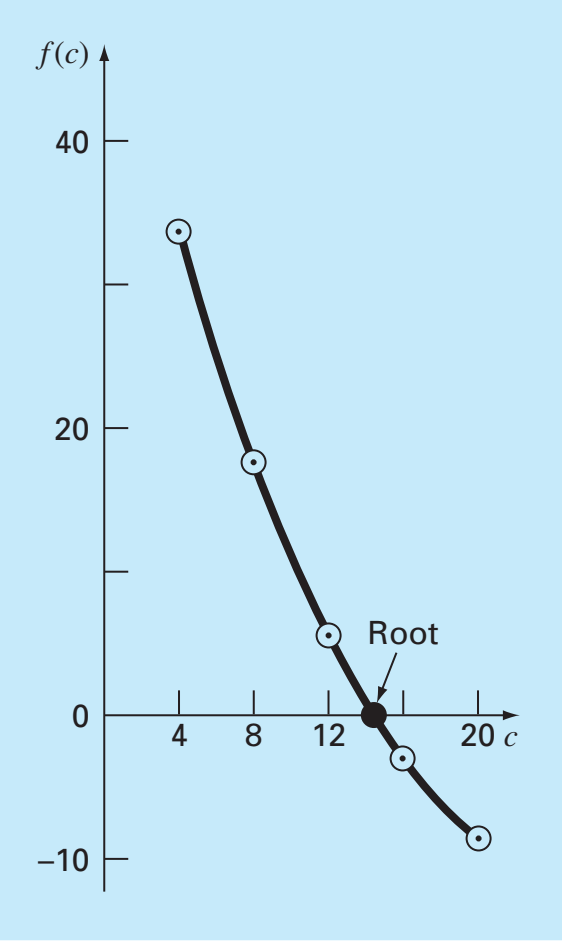
\includegraphics[height=0.8\textheight]{../chapra_7th/Chapra_Fig_5_1.png}
  \par}
\end{column}

\end{columns}



\end{frame}



\begin{frame}{Pembagian metode}
Secara garis besar, ada dua jenis metode yang akan dibahas:
\begin{itemize}\tightlist
\item Metode-metode pengurungan (\textit{bracketing}). Metode ini memerlukan
  dua titik awal sebagai tebakan posisi akar. Beberapa metode pengurungan:
  \begin{itemize}
  \item Metode bagi-dua (bisection)
  \item Metode regula-falsi
  \end{itemize}
\item Metode-metode terbuka. Metode ini hanya memerlukan satu titik awal sebagai
  tebakan posisi akar. Beberapa metode terbuka:
  \begin{itemize}
  \item Metode titik-tetap (fixed point)
  \item Metode Newton
  \item Metode secant
  \end{itemize}
\end{itemize}
\end{frame}


\begin{frame}{Metode bagi-dua (\textit{bisection})}

Metode bagi-dua bekerja dengan input tebakan awal $x_l$ dan $x_u$,
(dengan $x_l$ < $x_u$) yang
mengapit akar, artinya akar berada diantara $x_l$ dan $x_u$.
Jika $f(x)$ bernilai real dan kontinu dan
$$
f(x_l) f(x_u) < 0
$$
atau jika $f(x_l)$ dan $f(x_u)$ berbeda tanda maka ada
akar diantara $x_l$ dan $x_u$.
Untuk metode bagi-dua, tebakan akar diberikan oleh titik tengah
dari $x_l$ dan $x_u$:
$$
x_{r} = \frac{x_l + x_u}{2}
$$
Pada iterasi selanjutnya, salah satu dari $x_l$ dan $x_u$ akan
digantikan dengan $x_r$, bergantung dari tanda dari $f(x_r)$.

\end{frame}


\begin{frame}{Metode bagi-dua (\textit{bisection})}
Langkah-langkah metode bagi-dua:
\begin{itemize}\tightlist
\item STEP 1: Pilih $x_l$ dan $x_u$ yang memenuhi $f(x_l) f(x_u) < 0$
\item STEP 2: Hitung estimasi akar:
  \begin{equation*}
  x_r = \frac{x_l + x_u}{2}
  \end{equation*} 
\item STEP 3: Perbarui selang $[x_l, x_u]$:
  \begin{itemize}
  \item Jika $f(x_l) f(x_r) < 0$, ganti atau perbarui nilai $x_u \leftarrow x_r$
    kemudian kembali ke STEP 2.
  \item Jika $f(x_l) f(x_r) > 0$, ganti atau perbarui nilai $x_l \leftarrow x_r$
    kemudian kembali ke STEP 2.
  \item Jika $f(x_l) f(x_r) = 0$ atau nilai absolut dari $f(x_r)$ sudah lebih kecil
    dari nilai toleransi tertentu maka hentikan perhitungan.
  \end{itemize}
\end{itemize}

\end{frame}


\begin{frame}{Metode bagi-dua (\textit{bisection})}

{\centering
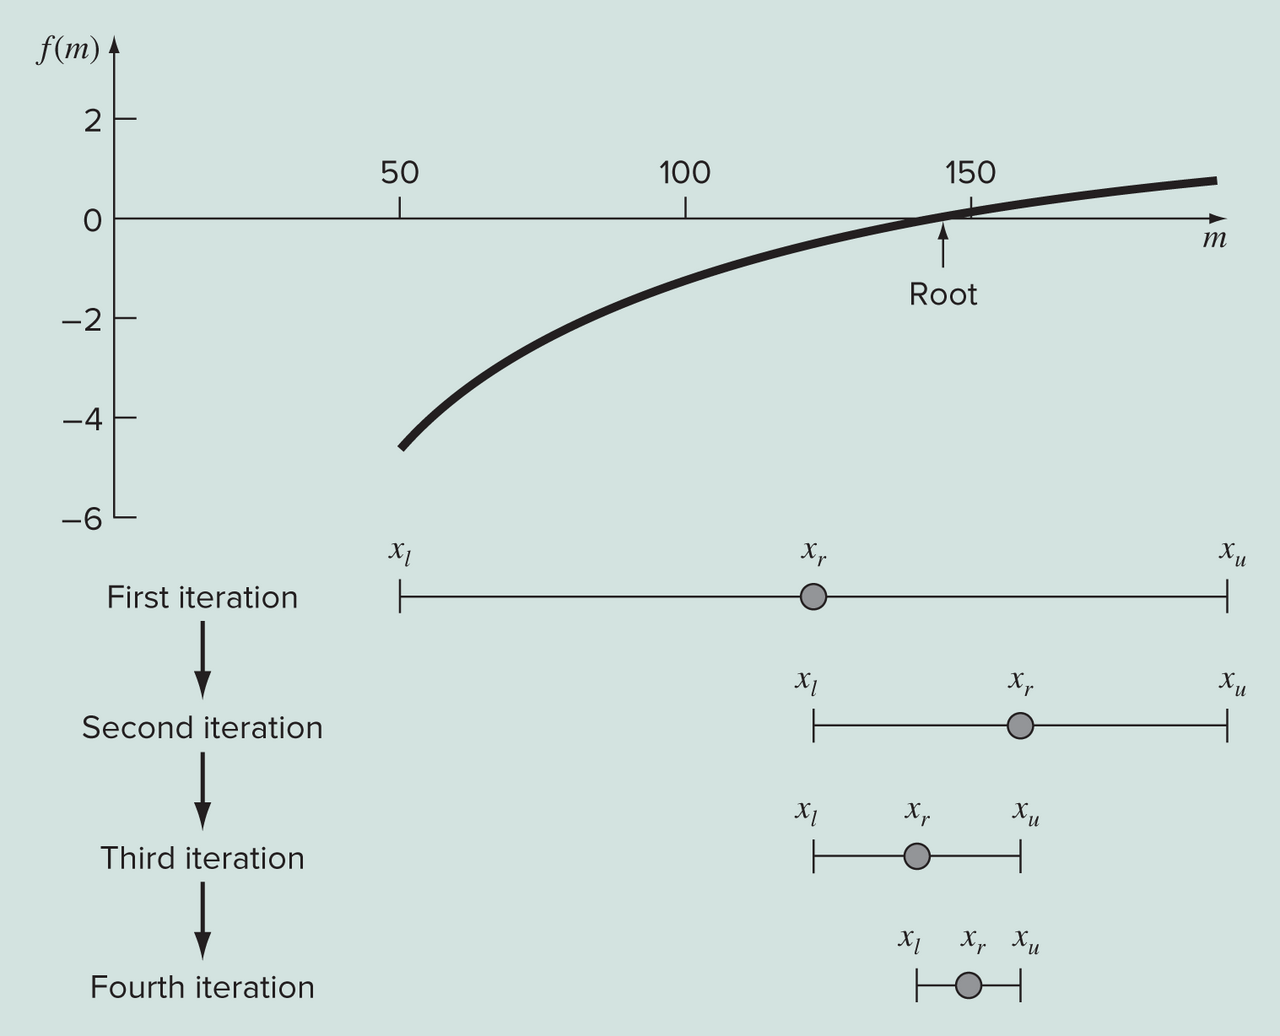
\includegraphics[height=0.8\textheight]{../chapra_python/Chapra_Fig_5_5.png}
\par}

\end{frame}


\begin{frame}{Contoh metode bagi-dua}

Contoh proses iterasi untuk $f(c)$ dengan tebakan selang $[12,16]$:

{\centering
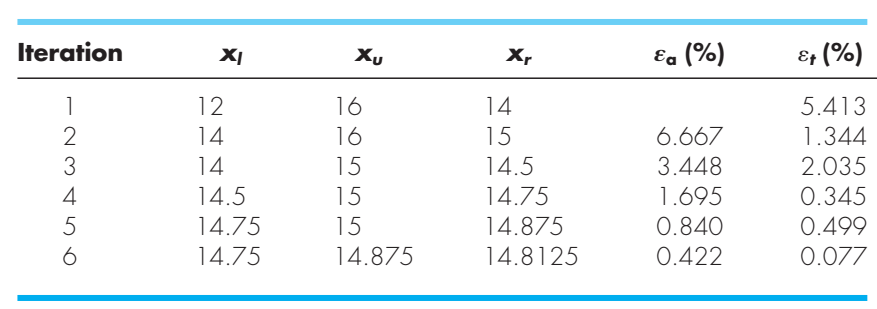
\includegraphics[height=0.5\textheight]{../chapra_7th/Chapra_Table_Example_5_4.png}
\par}

\end{frame}


\begin{frame}{Metode \textit{regula-falsi}}
\fontsize{9}{10}\selectfont

\begin{columns}
  
  \begin{column}{0.5\textwidth}
  Ide dari metode regula-falsi mirip dengan metode bagi-dua. Perbedaannya
  adalah estimasi akar diperoleh dari perpotongan garis lurus yang menghubungkan
  antara $f(x_l)$ dan $f(x_u)$ dengan sumbu-$x$.

  Dari gambar:
  $$
  \frac{f(x_l)}{x_r - x_l} = \frac{f(x_u)}{x_r - x_u}
  $$
  sehingga diperoleh:
  $$
  x_r = \frac{x_u f(x_l) - x_l f(x_u)}{f(x_l) - f(x_u)}
  $$
  atau (alternatif):
  $$
  x_r = x_u - \frac{f(x_u)(x_l - x_u)}{f(x_l) - f(x_u)}
  $$
  \end{column}

  \begin{column}{0.5\textwidth}
  {\centering
  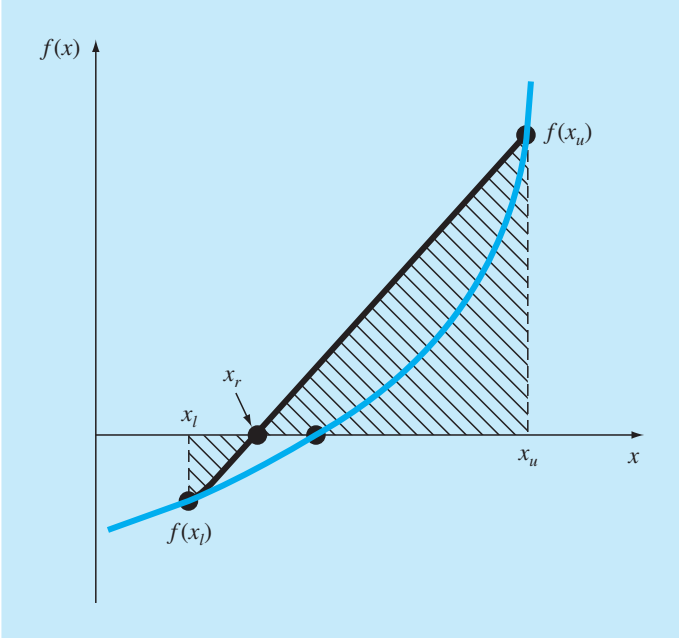
\includegraphics[height=0.7\textheight]{../chapra_7th/Chapra_Fig_5_12.png}
  \par}
  \end{column}

\end{columns}

\end{frame}


\begin{frame}{Metode \textit{regula-falsi}}
\fontsize{10}{11}\selectfont

\begin{columns}

  \begin{column}{0.5\textwidth}
  Implementasi metode \textit{regula-falsi} mirip dengan metode bagi-dua.
  Perbedaannya hanya pada persamaan yang digunakan untuk $x_r$.

  Biasanya metode \textit{regula-falsi} membutuhkan iterasi yang lebih sedikit
  untuk konvergen ke akar dibandingkan dengan metode bagi-dua, meskipun pada kasus
  tertentu metode bagi-dua dapat lebih cepat konvergen. Pada kasus ini, kita bisa
  mengatasinya dengan cara menggunakan metode bagi-dua jika konvergensi metode
  \textit{regula-falsi} stagnan setelah beberapa iterasi (Lihat Contoh 5.6 pada Chapra
  dan metode \textit{regula-falsi} yang dimodifikasi).
  \end{column}

  \begin{column}{0.5\textwidth}
  {\centering
  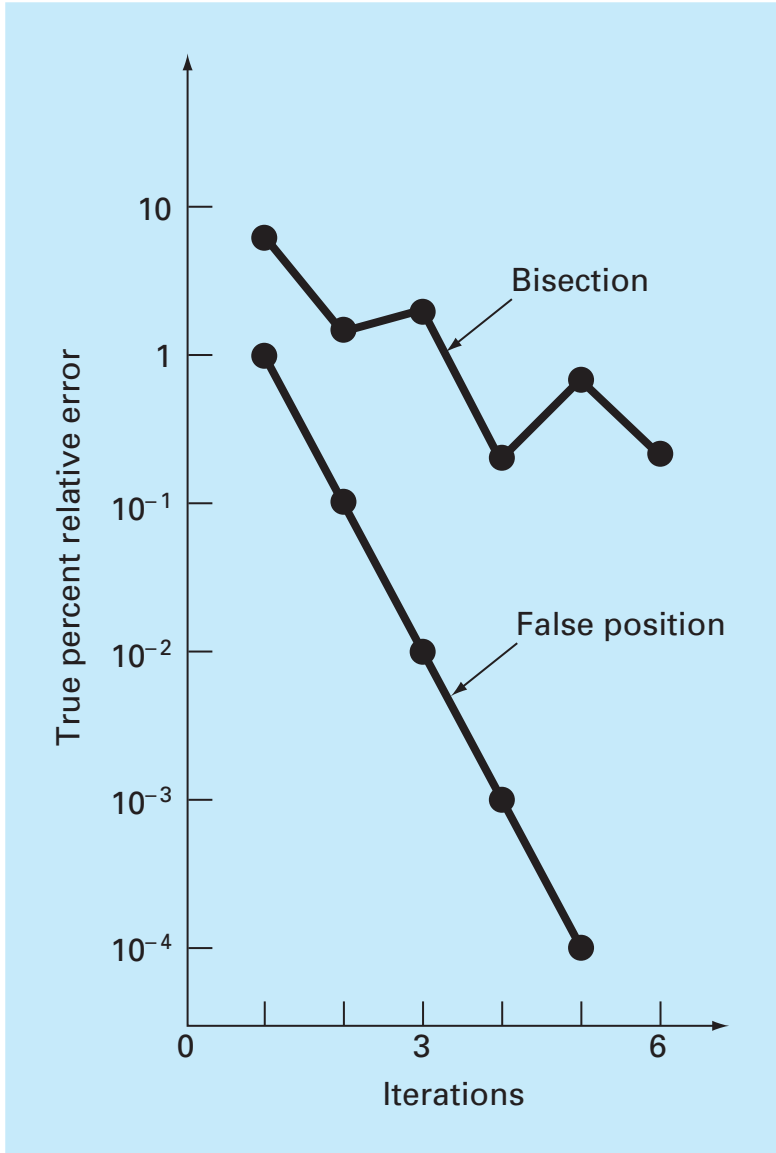
\includegraphics[height=0.8\textheight]{../chapra_7th/Chapra_Fig_5_13.png}
  \par}
  \end{column}

\end{columns}

\end{frame}

\begin{frame}{Metode iterasi titik-tetap (\textit{fixed-point} iteration)}
\fontsize{10}{11}\selectfont

Metode iterasi titik-tetap adalah salah satu dari metode terbuka untuk menghitung
akar dari persamaan nonlinear.
Langkah pertama dari metode ini adalah menuliskan kembali persamaan
$f(x) = 0$ menjadi:
\begin{equation}
x = g(x)  
\label{eq:x_gx}
\end{equation}
Jika $x$ merupakan akar dari $f(x)$ maka Persamaan \eqref{eq:x_gx}
juga akan terpenuhi. Artinya jika kita dapat menemukan $x$ sedemikan rupa sehingga
$x = g(x)$, maka kita telah menemukan akar dari $f(x)$.
Dalam bentuk iterasi, metode ini dapat dituliskan sebagai:
$$
x_{i+1} = g(x_{i})
$$
di mana $i$ adalah indeks iterasi. Terdapat beberapa kondisi yang dapat
digunakan untuk menentukan konvergensi. Salah satunya adalah dengan
menggunakan estimasi galat
$$
\epsilon_{a} = \left| \frac{x_{i+1} - x_{i}}{x_{i+1}} \right|
$$
Iterasi dihentikan jika $\epsilon_{a}$ lebih kecil dari suatu nilai
tertentu.
\end{frame}


\begin{frame}
\fontsize{9}{10}\selectfont

\begin{block}{Contoh metode iterasi titik-tetap}
Gunakan metode iterasi titik-tetap untuk mencari akar dari
$f(x) = e^{-x} - x$
\end{block}
Fungsi $f(x)$ diubah dulu mejadi $x = g(x)$ di mana $g(x) = e^{-x}$.
Iterasi titik-tetap memberikan skema iterasi:
$$
x_{i+1} = e^{-x_{i}}
$$
Dengan nilai awal $x_0 = 0$ diperoleh iterasi seperti pada tabel berikut.

{\centering
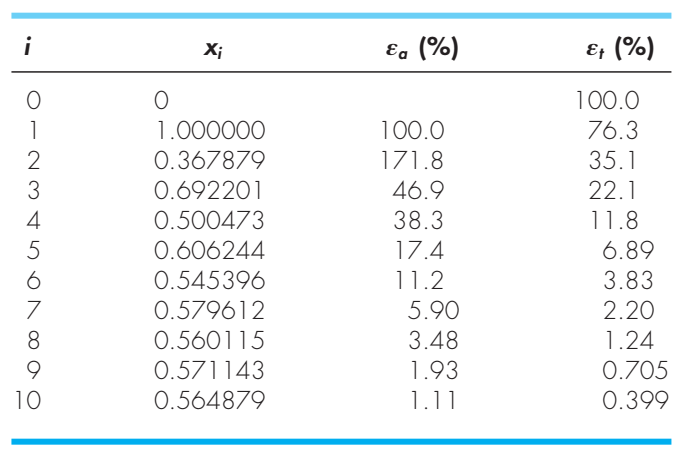
\includegraphics[height=0.5\textheight]{../chapra_7th/Chapra_Table_Example_6_1.png}
\par}

\end{frame}


\begin{frame}{Interpretasi grafis}
\fontsize{10}{11}\selectfont

\begin{columns}

  \begin{column}{0.5\textwidth}
  {\centering
  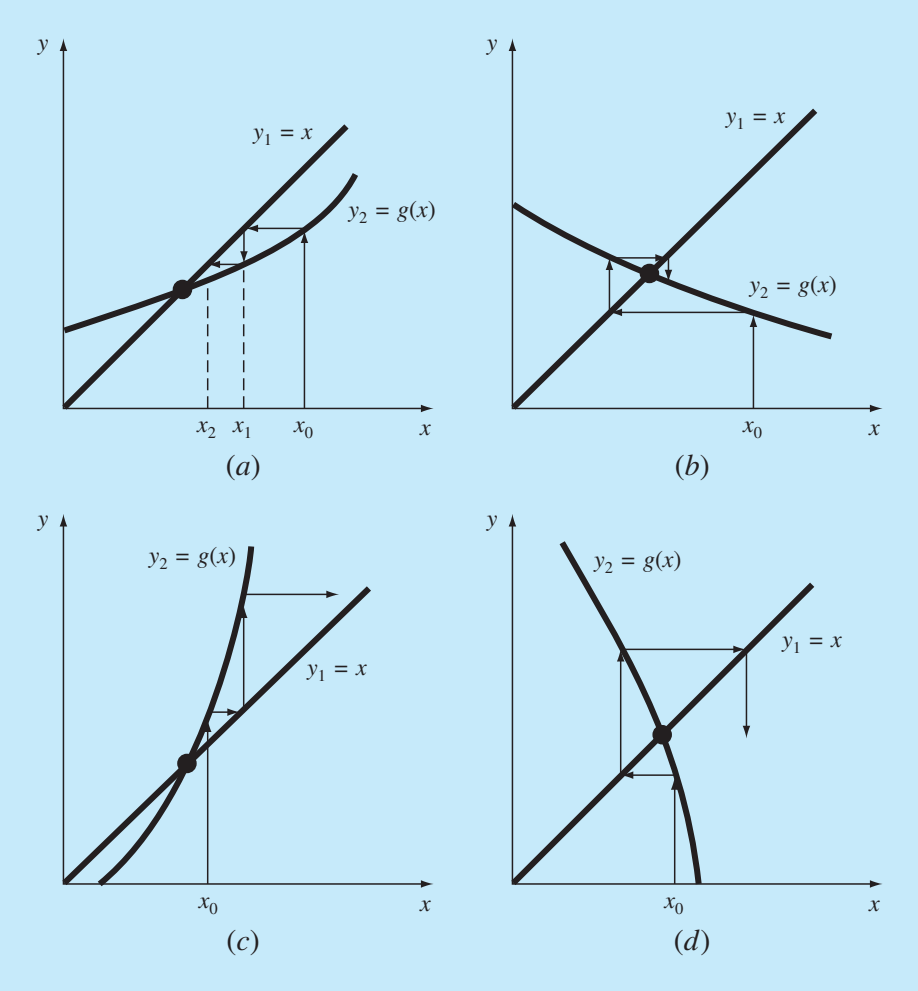
\includegraphics[height=0.8\textheight]{../chapra_7th/Chapra_Fig_6_3.png}
  \par}
  \end{column}

  \begin{column}{0.5\textwidth}
  Secara grafis, metode iterasi titik-tetap bertujuan untuk
  menemukan perpotongan antara kurva $y_1 = x$ dengan
  kurva $y_2 = g(x)$.

  Metode iterasi titik-tetap tidak selalu konvergen.

  Dari gambar, terlihat bahwa iterasi titik-tetap akan konvergen jika
  $|g'(x) < 1|$: magnitudo dari kemiringan $g(x)$ lebih kecil daripada
  kemiringan garis $y_1 = x$ pada daerah di mana metode ini diaplikasikan.
  \end{column}
\end{columns}

\end{frame}


\begin{frame}
\fontsize{9}{10}\selectfont

Skema iterasi:
$$
x_{i+1} = g(x_{i})
$$
Misalkan solusi dari iterasi titik-tetap ini adalah $x_r$, sehingga berlaku:
$$
x_{r} = g(x_r)
$$
Dengan mengurangi kedua persamaan tersebut diperoleh:
\begin{equation}
x_r - x_{i+1} = g(x_r) - g(x_i)
\label{eq:B6_1_1}
\end{equation}

Menggunakan teorema nilai rata-rata turunan: jika suatu fungsi $g(x)$
dan turunan pertamanya kontinu pada suatu interval $a \leq x \leq b$,
maka terdapat setidaknya satu nilai $x = \xi$ dalam interval tersebut
sedemikian rupa sehingga:
\begin{equation}
g'(\xi) = \frac{g(b) - g(a)}{b - a}
\label{eq:B6_1_2}  
\end{equation}
Ruas kanan dari persamaan ini adalah kemiringan dari garis yang menghubungkan antara
$g(a)$ dan $g(b)$. Dengan kata lain, teorema rata-rata turunan menyatakan bahwa
setidaknya ada satu titik di antara $a$ dan $b$ yang memiliki kemiringan,
$g'(\xi)$, yang sejajar dengan garis yang menghubugkan antara $g(a)$ dan
$g(b)$.
\end{frame}


\begin{frame}
\fontsize{9}{10}\selectfont

Jika $a = x_{i}$ dan $b = x_r$, maka ruas kanan dari
Persamaan \eqref{eq:B6_1_1} dapat dituliskan sebagai:
\begin{equation*}
g(x_r) - g(x_i) = (x_r - x_i) g'(\xi)
\end{equation*}
sehingga Persamaan \eqref{eq:B6_1_1} dapat dituliskan juga menjadi:
\begin{equation}
x_r - x_{i+1} = (x_r - x_i) g'(\xi)
\end{equation}
Dengan definisi galat sebenarnya untuk iterasi ke-$i$ sebagai:
$$
E_{t,i} = x_r - x_i
$$
maka:
$$
E_{t,i+1} = g'(\xi) E_{t,i}
$$
Dari persamaan ini dapat dilihat bahwa galat akan semakin berkurang pada
setiap iterasi jika $|g'(x)| < 1$. Sebaliknya, jika $|g'(x)| > 1$
galat akan semakin membesar.

Selain itu, jika turunan bernilai positif, maka galat akan positif solusi iteratif
akan monotonik. Jika turunan bernilai negatif, maka galat akan berosilasi.

Analisis ini juga menunjukkan bahwa galat pada metode iterasi titik-tetap akan
sebanding dengan galat dari langkah sebelumnya. Oleh karena ini iterasi titik-tetap
dikatakan memiliki sifat konvergensi linear (\textit{linearly convergent}).
\end{frame}


\begin{frame}{Metode Newton-Raphson}
\fontsize{9}{10}\selectfont

\begin{columns}

  \begin{column}{0.5\textwidth}
  Metode Newton-Raphson mungkin adalah metode yang paling terkenal
  di antara metode pencarian akar linear.

  Pada metode ini jika kita mulai dari tebakan akar $x_i$, kita dapat menarik garis
  singgung (\textit{tangent line})
  dari titik $(x_i, f(x_i))$. Titik perpotongan antara garis singgung ini
  dengan sumbu-$x$ merupakan tebakan selanjutnya untuk akar.
  
  Dari gambar dapat dicari garis singgung pada $x_i$:
  $$
  f'(x_{i}) = \frac{f(x_i) - 0}{x_i - x_{i+1}}
  $$
  diperoleh:
  \begin{equation}
  \myhighlight{
  x_{i+1} = x_{i} - \frac{f(x_{i})}{f'(x_{i})}
  }\label{eq:Chapra_6_6}
  \end{equation}
  Metode ini dapat digunakan jika $f'(x_{i}) \neq 0$.
  \end{column}

  \begin{column}{0.5\textwidth}
  {\centering
  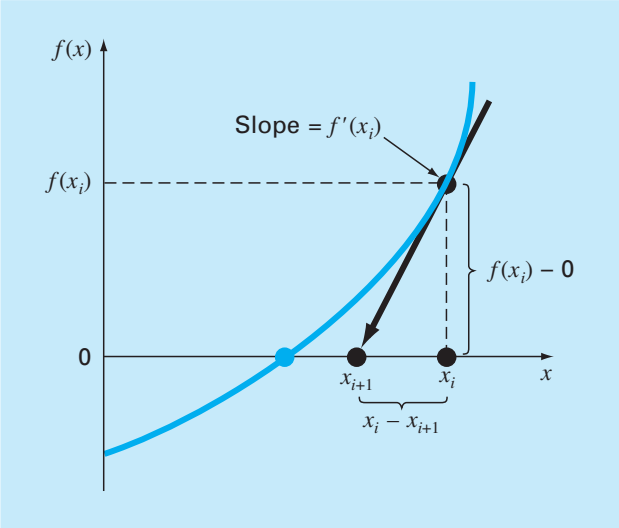
\includegraphics[height=0.8\textheight]{../chapra_7th/Chapra_Fig_6_5.png}
  \par}
  \end{column}

\end{columns}

\end{frame}


\begin{frame}
\fontsize{10}{11}\selectfont

\begin{block}{Contoh}
Gunakan metode Newton-Raphson untuk mengestimasi akar dari $f(x) = e^{-x} - x$ dengan
menggunakan tebakan akar awal $x_{0} = 0$.
\end{block}

Kita perlu mencari $f'(x)$ terlebih dahulu:
$$
f'(x) = -e^{-x} - 1
$$
Dengan menggunakan skema iterasi pada Persamaan \eqref{eq:Chapra_6_6} diperoleh
hasil pada tabel berikut.

{\centering
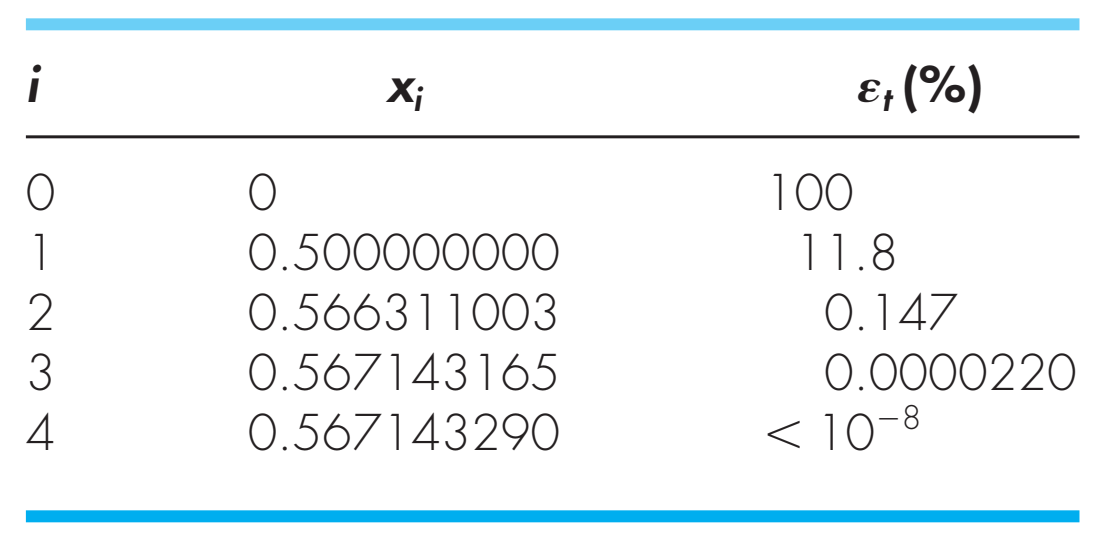
\includegraphics[height=0.4\textheight]{../chapra_7th/Chapra_Table_Example_6_3.png}
\par}

\end{frame}


\begin{frame}
\fontsize{9}{10}\selectfont

\begin{columns}
  \begin{column}{0.5\textwidth}
  \begin{block}{Contoh}
  Tentukan akar positif dari $f(x) = x^{10} - 1$ dengan menggunakan metode Newton-Raphson
  dan tebakan awal $x_0 = 0.5$.
  \end{block}
  Biasanya metode Newton-Raphson konvergen ke akar dengan cepat (konvergensi kuadratik).
  Namun pada kasus tertentu, seperti pada contoh ini,
  metode Newton-Raphson dapat kesulitan untuk konvergen.
  
  Skema iterasi Newton-Raphson pada kasus ini dapat dituliskan sebagai berikut:
  $$
  x_{i+1} = x_{i} - \frac{x_{i}^{10} - 1}{10x_{i}^{9}}
  $$
  Diperoleh hasil pada tabel berikut.
  \end{column}

  \begin{column}{0.5\textwidth}
  
  {\centering
  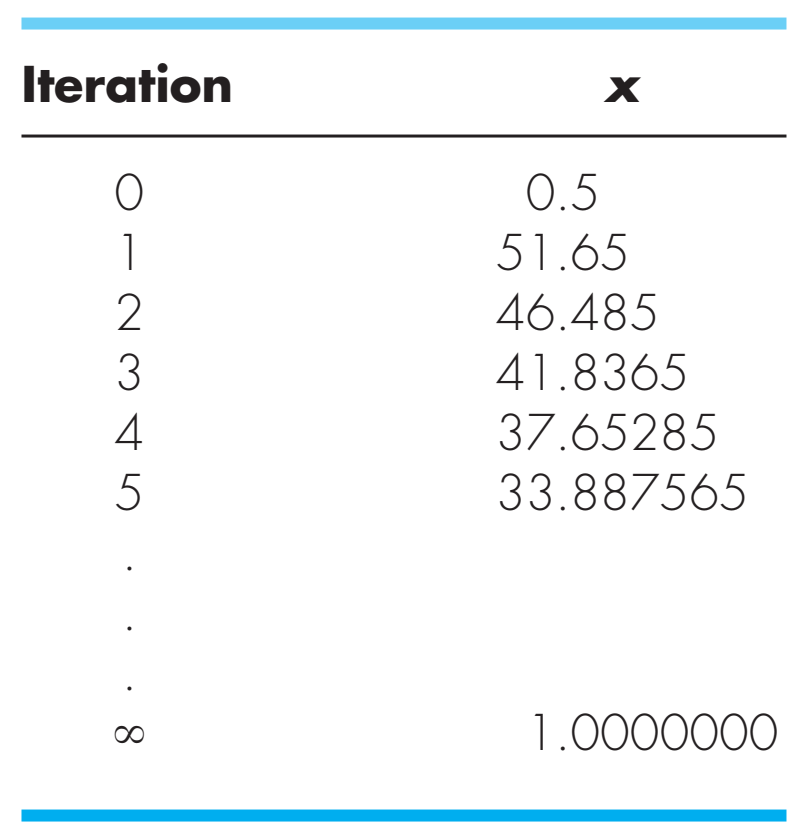
\includegraphics[height=0.5\textheight]{../chapra_7th/Chapra_Table_Example_6_5.png}
  \par}

  Seperti terlihat pada tabel, metode Newton-Raphson konvergen sangat lambat ke
  akar.

  Penyebab dari konvergensi yang lambat ini dapat didiagnosa
  dengan cara membuat plot dari fungsi yang bersangkutan.
  Biasanya dapat terjadi osilasi atau nilai tebakan akar yang
  jelek dikombinasikan dengan turunan fungsi yang sangat kecil
  (garis singgung yang hampir sejajar dengan sumbu-$x$)
  dapat membuat metode Newton-Raphson kesulitan untuk konvergen.

  \end{column}

\end{columns}

\end{frame}


\begin{frame}{Metode garis-potong (\textit{secant})}

Metode garis-potong mirip dengan metode Newton-Raphson. Perbedaannya
adalah pada metode garis-potong, turunan fungsi diaproksimasi dengan menggunakan
beda-hingga mundur:
$$
f'(x_{i}) \approx \frac{f(x_{i-1}) - f(x_i)}{x_{i-1} - x_{i}}
$$
sehingga diperoleh skema iterasi:
$$
x_{i+1} = x_{i} - \frac{f(x_{i}) (x_{i-1} - x_{i})}{f(x_{i-1}) - f(x_{i})}
$$
Metode garis potong memerlukan dua titik untuk memulai iterasi. Berbeda dengan
metode tertutup, dua titik ini tidak perlu mengapit akar.

\end{frame}



\begin{frame}{Metode garis-potong modifikasi}

Pada metode ini tidak digunakan dua tebakan awal, namun hanya satu titik saja.
Untuk mengaproksimasi turunan, digunakan gangguan kecil:
$$
f'(x_i) \approx \frac{f(x_i + \delta \, x_{i}) - f(x_i)}{\delta \, x_{i}}
$$
atau:
$$
x_{i+1} = x_{i} - \frac{\delta \, x_{i} f(x_i)}{f(x_{i} + \delta \, x_i) - f(x_i)}
$$
dengan $\delta$ adalah suatu bilangan fraksional yang kecil, misalnya $10^{-5}$.

Alternatif lain adalah dengan mengganti keseluruhan $\delta x_{i}$
dengan suatu konstanta yang kecil.

\end{frame}


\begin{frame}{Metode-metode lain}

Selain dari metode-metode yang telah disebutkan sebelumnya, juga
terdapat banyak metode-metode lain yang dapat digunakan untuk mencari
akar persamaan nonlinear:
\begin{itemize}\tightlist
\item Modifikasi metode Newton
\item Metode Brent
\item Metode Muller
\item Metode Ridder
\end{itemize}

\end{frame}


\begin{frame}{Pustaka SciPy}

Akar nonlinear

\end{frame}



\begin{frame}{Beberapa catatan}
\begin{itemize}
\item Plotting
\end{itemize}
\end{frame}




\begin{frame}{Sistem Persamaan Nonlinear}
\begin{align*}
f_{1} (x_1, x_2, \ldots, x_n) & = 0 \\
f_{2} (x_1, x_2, \ldots, x_n) & = 0 \\
\cdots \\
f_{n} (x_1, x_2, \ldots, x_n) & = 0
\end{align*}
\end{frame}

\end{document}
